% Author: Daniel Celis Garza <daniel.celisgarza@materials.ox.ac.uk>
% Date of creation: 2017/03/09
% Last edit: 2017/03/09

% Preamble with all the basic packages a thesis would need. Modify as needed.

\documentclass[htwologo,twosup,12pt]{genthesis}
% By changing the document class this preamble can be used for other document types.
% genthesis.cls contains the definition of the document class.
% Geometry
\usepackage[top=1in, bottom=1in, 
outer=1in, inner=1in] % inner = 1.5 for binding
{geometry}

%----------------------- Fonts, symbols and colours ------------------------%
% If using pdfLaTeX comment fontspec and uncomment fontenc and inputenc. If using the superior XeLaTeX/XeTeX or LuaTeX do the opposite.
\usepackage{fontspec}					% XeLaTeX & LuaTeX fonts.
%\usepackage[T1]{fontenc}				% Font encoding for pdfLaTeX
%\usepackage[latin1]{inputenc}			% Input encoding (easy accents) for pdfLaTeX
\usepackage{amssymb, amsmath,
	bm	   , isomath,
	mathtools}					% Maths fonts and symbols.
\usepackage{exscale}					% Removes the need to use {\displaystyle }.
%\newfontfamily\ubuntumono{Ubuntu Mono} % Ubuntu font for fancy shell commands (font needs to be installed).
\usepackage{xcolor}
%\definecolor{oxfordblue}{cmyk}{79,56,0,72}
\definecolor{oxfordblue}{RGB}{15,31,71}
\usepackage{lmodern}

%------------------------ Hyperlinks and references ------------------------%
\usepackage[colorlinks     = true, % Hyperlinks.
pdfstartview   = FitV,
linkcolor      = oxfordblue,
citecolor      = oxfordblue,
urlcolor       = oxfordblue,
hyperfootnotes = true,
hypertexnames  = true,
plainpages     = false % Correctly links index entries whenever \thispagestyle{empty} is used.
]{hyperref}
\usepackage[comma  , square,       % Citing style.
numbers, sort&compress
]{natbib}
\usepackage{cleveref} 			   % Automatic referencing better than \autoref{}.

%--------------------------- Index and glossary ----------------------------%
\usepackage{makeidx} % Index.
\usepackage{xparse}	 % Expanded macro capability.
\makeindex			 % Creates index.
\usepackage[toc, acronyms
]{glossaries} % Glossary.
\setglossarystyle{altlisthypergroup} % Sets a list of letters with hyperlinks before the glossaries and acronyms.
% Dual glossary entry.
% Define dual entry for glossary + acronym.
% https://en.wikibooks.org/wiki/LaTeX/Glossary#Dual_entries_with_reference_to_a_glossary_entry_from_an_acronym
% Syntax: \newdualentry[glossary options][acronym options]{label}{abbrv}{long}{description}
\DeclareDocumentCommand{\newdualentry}{ O{} O{} m m m m } {
	\newglossaryentry{gls-#3}{name={#5},text={#5\glsadd{#3}},
		description={#6},#1
	}
	\makeglossaries
	\newacronym[see={[Glossary:]{gls-#3}},#2]{#3}{#4}{#5\glsadd{gls-#3}}
}

%--------------------------------- Utility ---------------------------------%
\usepackage{setspace}  % Text spacing commands.
%\usepackage{paralist} % In-paragraph lists.
%\usepackage{pdfpages} % Include pdf pages.
%\usepackage{lscape}   % Use landscape pages.
%\allowdisplaybreaks   % Math environments continue onto the next page if they overflow.
\usepackage{siunitx}   % International units.
\usepackage{hologo}    % XeLaTeX and BibTex logos.

%--------------------------------- Floats ----------------------------------%
%\usepackage{float} 			% Extra options for floats.
%\usepackage[section]{placeins} % Force floats to stay in the sections they're called in.
\usepackage{booktabs} 			% Nicer tables.
%\usepackage{multirow} 			% Multirow and multicolumn tables. Avoid when possible.
\usepackage{subcaption} 		% Subfigures.
%\usepackage{epstopdf} 			% pdfLaTeX does not support eps images so they need to be converted to pdf.

%---------------------------- Scripts and code -----------------------------%
% If you only need basic script support use verbatim. If you want more features use listings. If you can install pygments use minted.
%\usepackage{verbatim} % Type commands without the hassle of the other two.
%\usepackage{listings} % Spartan display of code and pseudo code.
\usepackage{minted}   % Elegantly display code. Requires a Python 2.7 or higher installation of pygments to be installed. Requires "-shell-escape" flag to the LaTeX compilation command.
\usepackage[chapter]{algorithm}
\usepackage{algpseudocode} % Package for algorithm typesetting (pseudo-code).

%---------------------------- Image file paths -----------------------------%
\graphicspath{{./images/}}

%------------------------------- Input files -------------------------------%
\newcommand{\kwdmc}[2]{\gls{#1}\index{\ensuremath{#2}}} % Keyword math command.
\newcommand{\kwdm}[1]{\gls{#1}\index{\ensuremath{#1}}}  % Keyword math.
\newcommand{\kwd}[1]{\gls{#1}\index{#1}}				% Keyword.
\newcommand{\incarabcounter}{							% Preserves arabic numbering before using the romanpages environment.
	\setcounter{arabiccounter}{\value{page}}
	%
	\if@twocolumn
		\addtocounter{arabiccounter}{1}
	\else
		\if@openright
			\addtocounter{arabiccounter}{2}
		\else
			\addtocounter{arabiccounter}{1}
		\fi
	\fi
}	 % Macros.
\newglossaryentry{pi}
{
	name = {\ensuremath{\pi}},
	description = {Ratio of circumference of circle to its
		diameter},
	sort = pi
}
\newglossaryentry{e}
{
	name = {\ensuremath{e}},
	description = {Euler's number defined as \ensuremath{\lim\limits_{n\to\infty} \left(1 + \dfrac{1}{n}\right)^{n}}}
}
\newglossaryentry{tensor}
{
	name={tensor},
	description={Geometric object that describes linear relations between geometric vectors, scalars and other tensors. They are generalisations of scalars (no indices), vectors (one index) and matrices (two indices) to $ n $ indices},
	plural=tensors
} % Glossaries.

%----------------------------- Special options -----------------------------%
%\counterwithout{figure}{chapter} % Uncomment to remove chapter number from figures.
%\counterwithout{table}{chapter}  % Uncomment to remove chapter number from tables.
%\setlength{\topskip}{0in}        % Top paragraph spacing.
%\setlength{\parskip}{2ex}        % Bottom paragraph spacing.
%\linespread{1.5} 				  % Inter-line spacing (1 = single space, 1.5 = double space).
%\renewcommand{\footnoterule}{% Footnote fule that spans the whole textwidth.
%	\kern -5.4pt
%	\hrule width \textwidth height 0.4pt
%	\kern 5pt
%}
%\makeatletter \newcommand*{\codefont}{% \codefont provides font size for code (for use in listings and minted).
%	\@setfontsize
%	\codefont{10pt}{11pt}
%}\makeatother
\begin{document}
%-----------------------------------------
%                 Header
%-----------------------------------------
\himage{\paperwidth}{header.pdf}
\begin{flushleft}
	\begin{minipage}{0.9\paperwidth}
		\centering
		{\fontsize{72}{86.4}\color{white}\selectfont\textbf{\emph{GPU Implementation of the Analytical Integration of\\ Forces Induced by Dislocations on Surface Elements}}}\\[0.8cm]
		{\fontsize{48}{57.6}\color{white}\selectfont\textbf{\emph{Daniel Celis Garza\textsuperscript{*1}, Edmund Tarleton\textsuperscript{1}, Angus Wilkinson\textsuperscript{1}}}}\\[0.6cm]
		{\fontsize{48}{57.6}\color{white}\selectfont\textbf{\emph{\textsuperscript{1}Department of Materials, University of Oxford, Parks Rd, Oxford OX1 3PH}}}\\[0.6cm]
		{\fontsize{48}{57.6}\color{white}\selectfont\textbf{\emph{\textsuperscript{*}E-mail: \texttt{daniel.celisgarza@materials.ox.ac.uk}}}}
	\end{minipage}
\end{flushleft}
\vspace{5cm}
\begin{multicols}{2}
	%
	{\fontsize{37}{44.4}\selectfont
	\section{Introduction}
	%
		The assumption of an asymptotically infinite crystalline matrix, greatly limits the applicability and scalability of Discrete Dislocation Dynamics (DDD) simulations.
		
		In order for DDD simulations to be more widely used in scientific and engineering applications (fig. \ref{f:dislocation}), a way must be found to simulate finite volumes.
		\scfloat{0cm}{.525\linewidth}%
		{%
			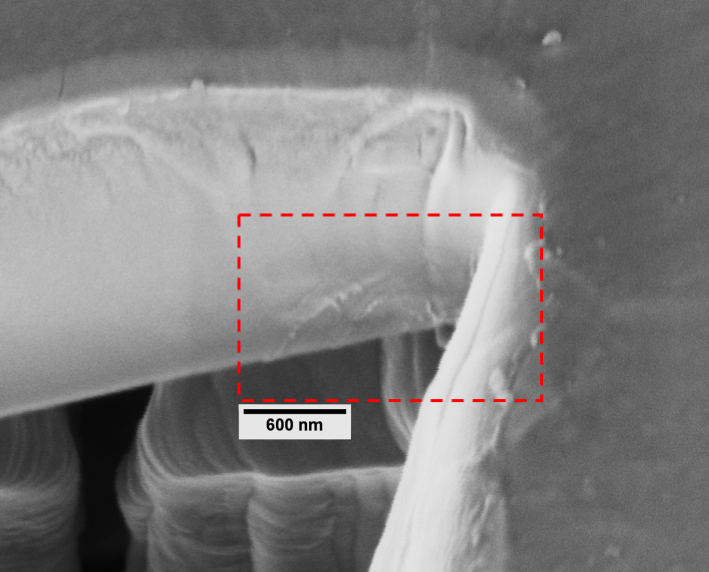
\includegraphics[width=\linewidth]{dislocation.png}
		}{\quad}{.425\linewidth}
		{%
			\captionof{figure}{Bent microcantilever test. The plastic deformation of materials is mediated by the nucleation and motion of dislocations. The red box contains slip steps due to dislocations exiting at the free surface. Image kindly provided by Bo-Shiuan Li.}
			\label{f:dislocation}
		}{0cm}
				
		This is often done by decomposing the problem into two steps as shown in eq. \ref{e:stress} and fig. \ref{f:fem_ddd}. Given the initial traction conditions $ \bm{T_{0}} $. The stress field produced by the dislocation ensemble, $ \sum_{\textrm{d}} \bm{\tilde{\sigma}}_{\textrm{d}} $, is used to calculate a corrective stress field, $ \bm{\hat{\sigma}} $, produced by the boundaries. The resultant stress is the sum of both stress fields,
		\begin{align}
			\bm{\sigma} = \bm{\hat{\sigma}} + \sum\limits_{\textrm{d}} \bm{\tilde{\sigma}}_{\textrm{d}}\,.\label{e:stress}
		\end{align}
		\cfloat{1cm}{0.95\linewidth}%
		{%
			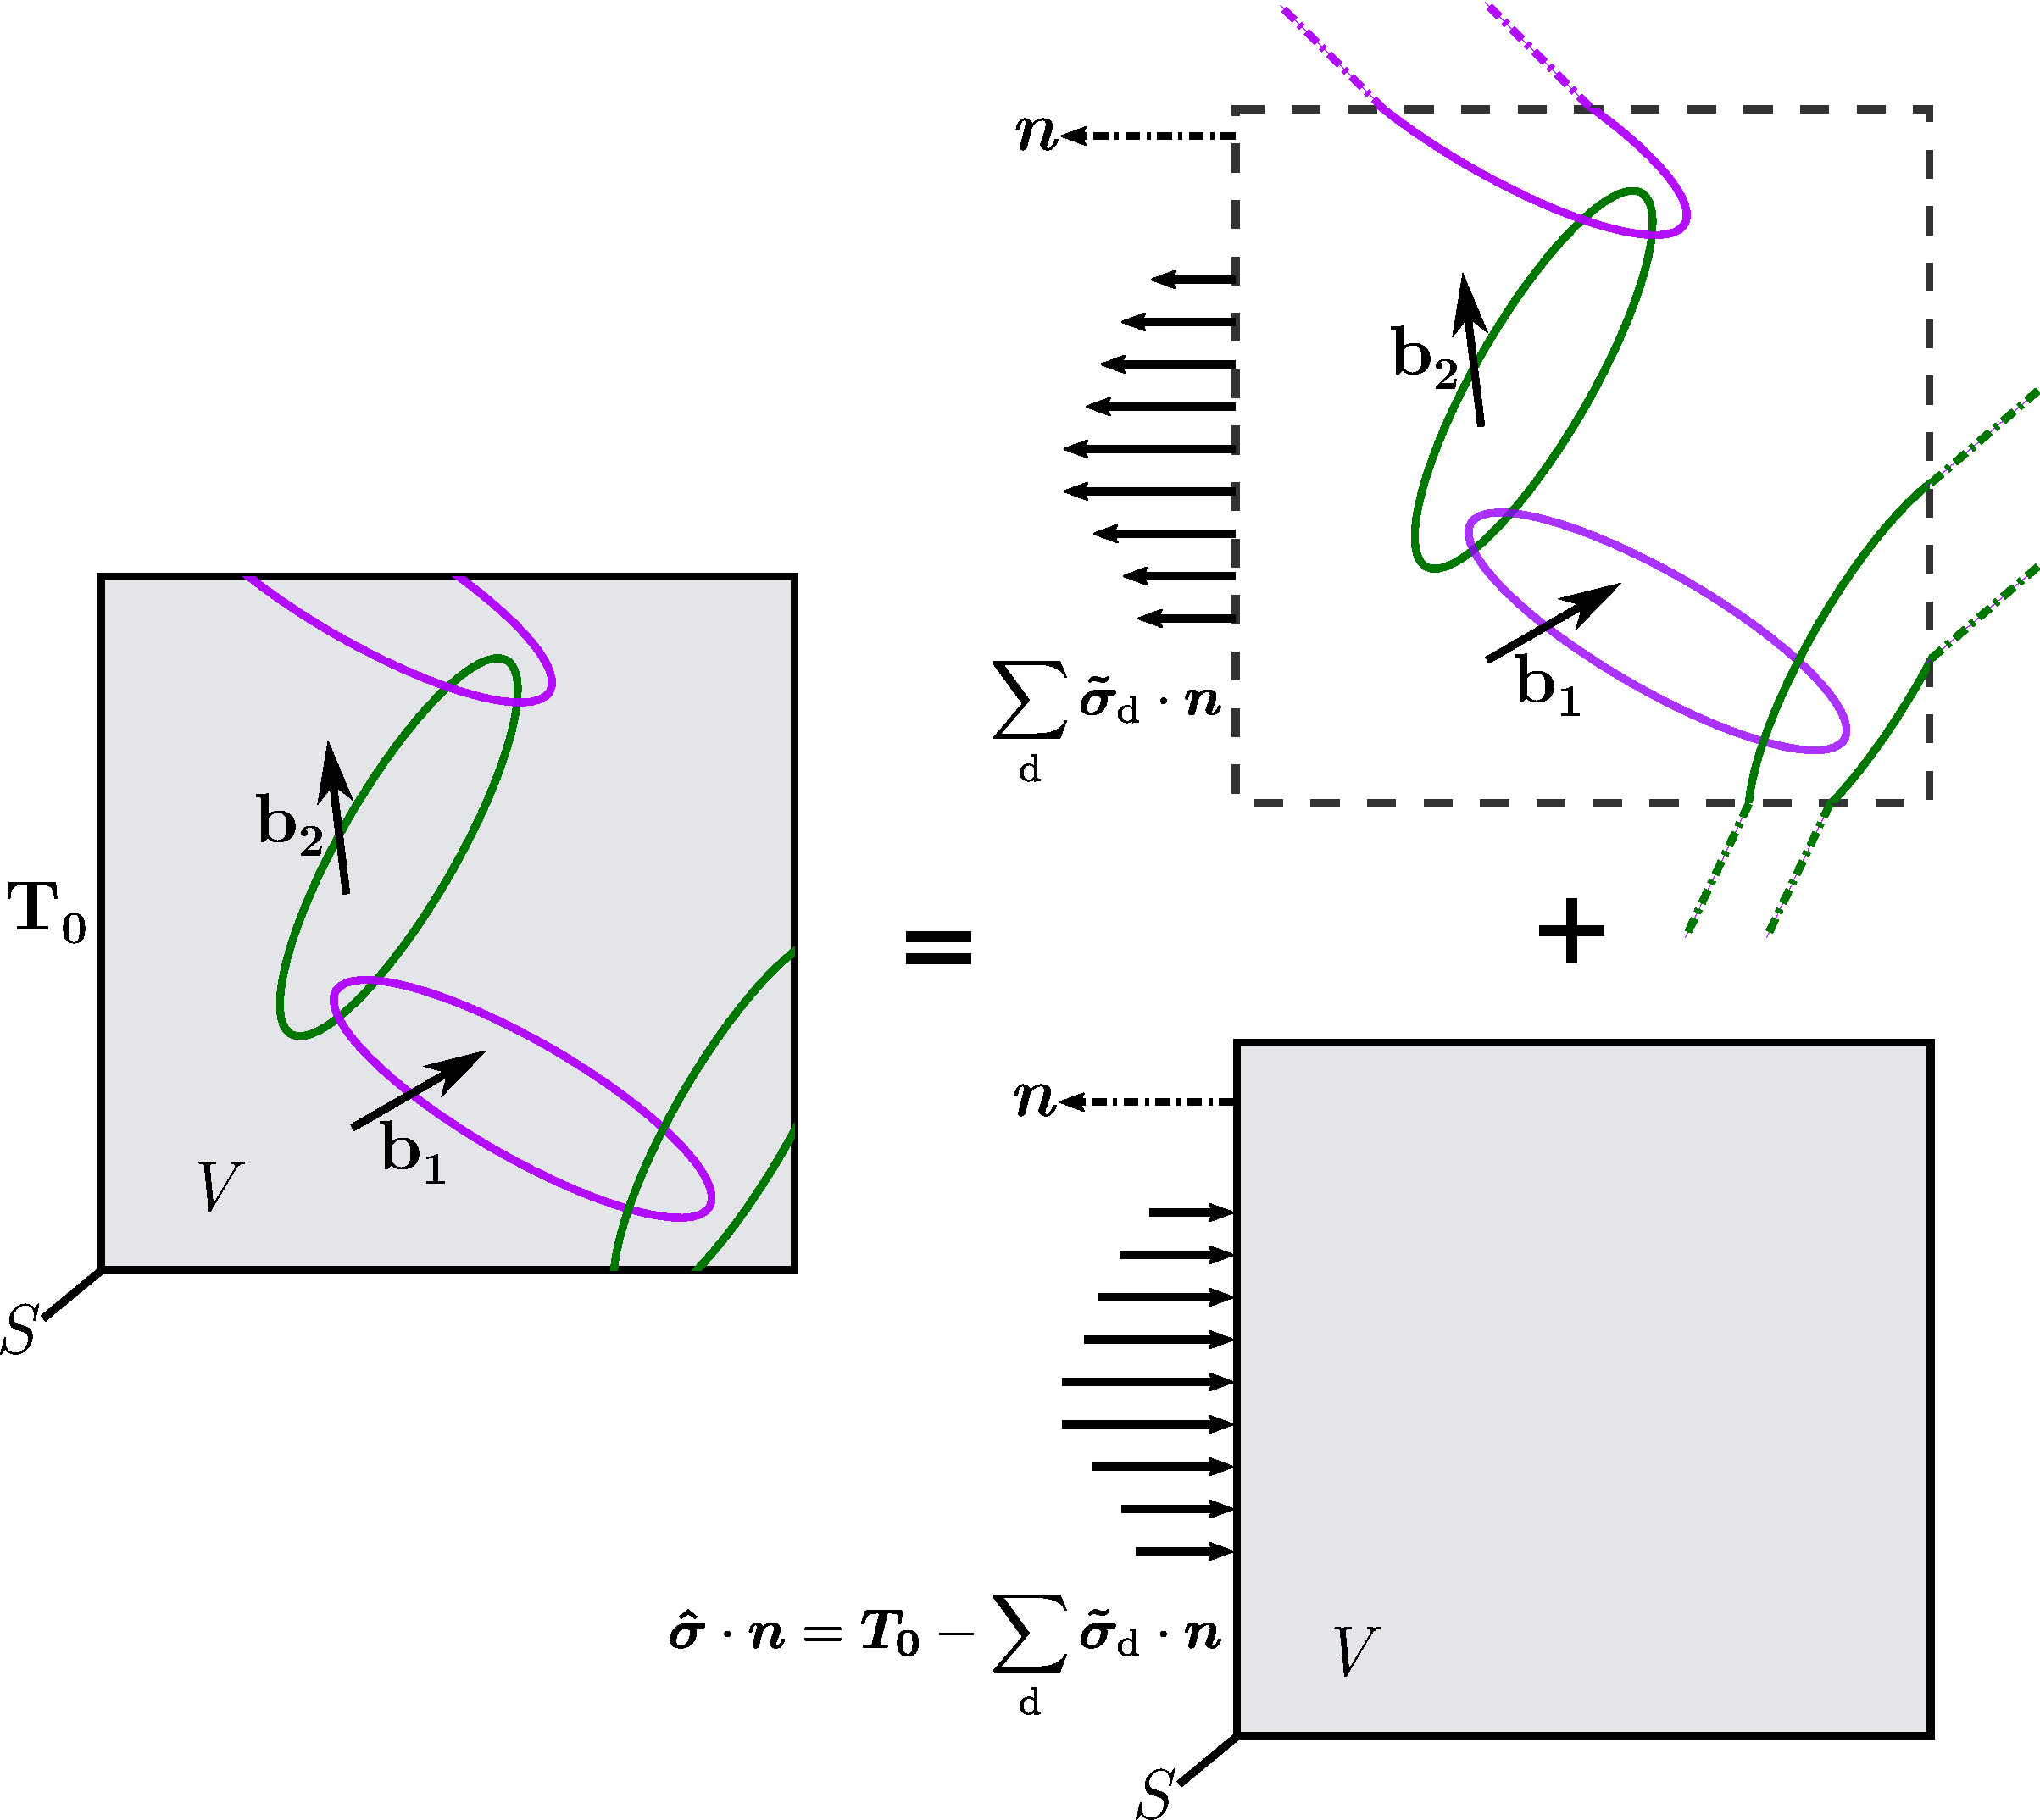
\includegraphics[width=\linewidth]{fem_ddd.pdf}% picture filename
			\captionof{figure}{The dislocation ensemble in a volume V is bounded by a surface S. First, the traction field $ \sum_{\textrm{d}} \bm{\tilde{\sigma}}_{\textrm{d}} $ due to the dislocation ensemble is evaluated at the surface. Then, a traditional FE or BE simulation calculates the image traction field $ \bm{\hat{\sigma}} \cdot \bm{n} $. Which is then used to evolve the dislocation positions and repeat the cycle. Image edited from \cite{analytical_integration_of_the_forces_induced_by_dislocations_on_a_surface_element}.}
			\label{f:fem_ddd}
		}{1cm}
		This means we must evaluate the forces upon a surface by the dislocation loop ensemble. Doing so numerically is problematic because error minimisation is very computationally expensive due to poor scaling.
		
		\citet{analytical_integration_of_the_forces_induced_by_dislocations_on_a_surface_element} have found an analytical solution to this problem, which is to be implemented on NVidia Graphics Cards using CUDA C and used as part of the DDLab code.
	%
	\section{Methodology}
	%
		The solution consists on solving 44 triple integrals via recurrence relations and 6 seed functions. This solution has scaling $ O(1) $ as there are no quadrature points, and is exact in both the finite and asymptotically infinite domains. The expressions are outside the scope of this poster and can be found in \cite{analytical_integration_of_the_forces_induced_by_dislocations_on_a_surface_element}.
		
		In essence, the main idea behind the solution can be found in fig. \ref{f:force_calc}. Where the stress field for non-singular dislocations \cite{a_non-singular_continuum_theory_of_dislocations} is weighted by linear shape functions that linearly distribute the nodal load on the surface element.
		\cfloat{1cm}{0.95\linewidth}%
		{%
			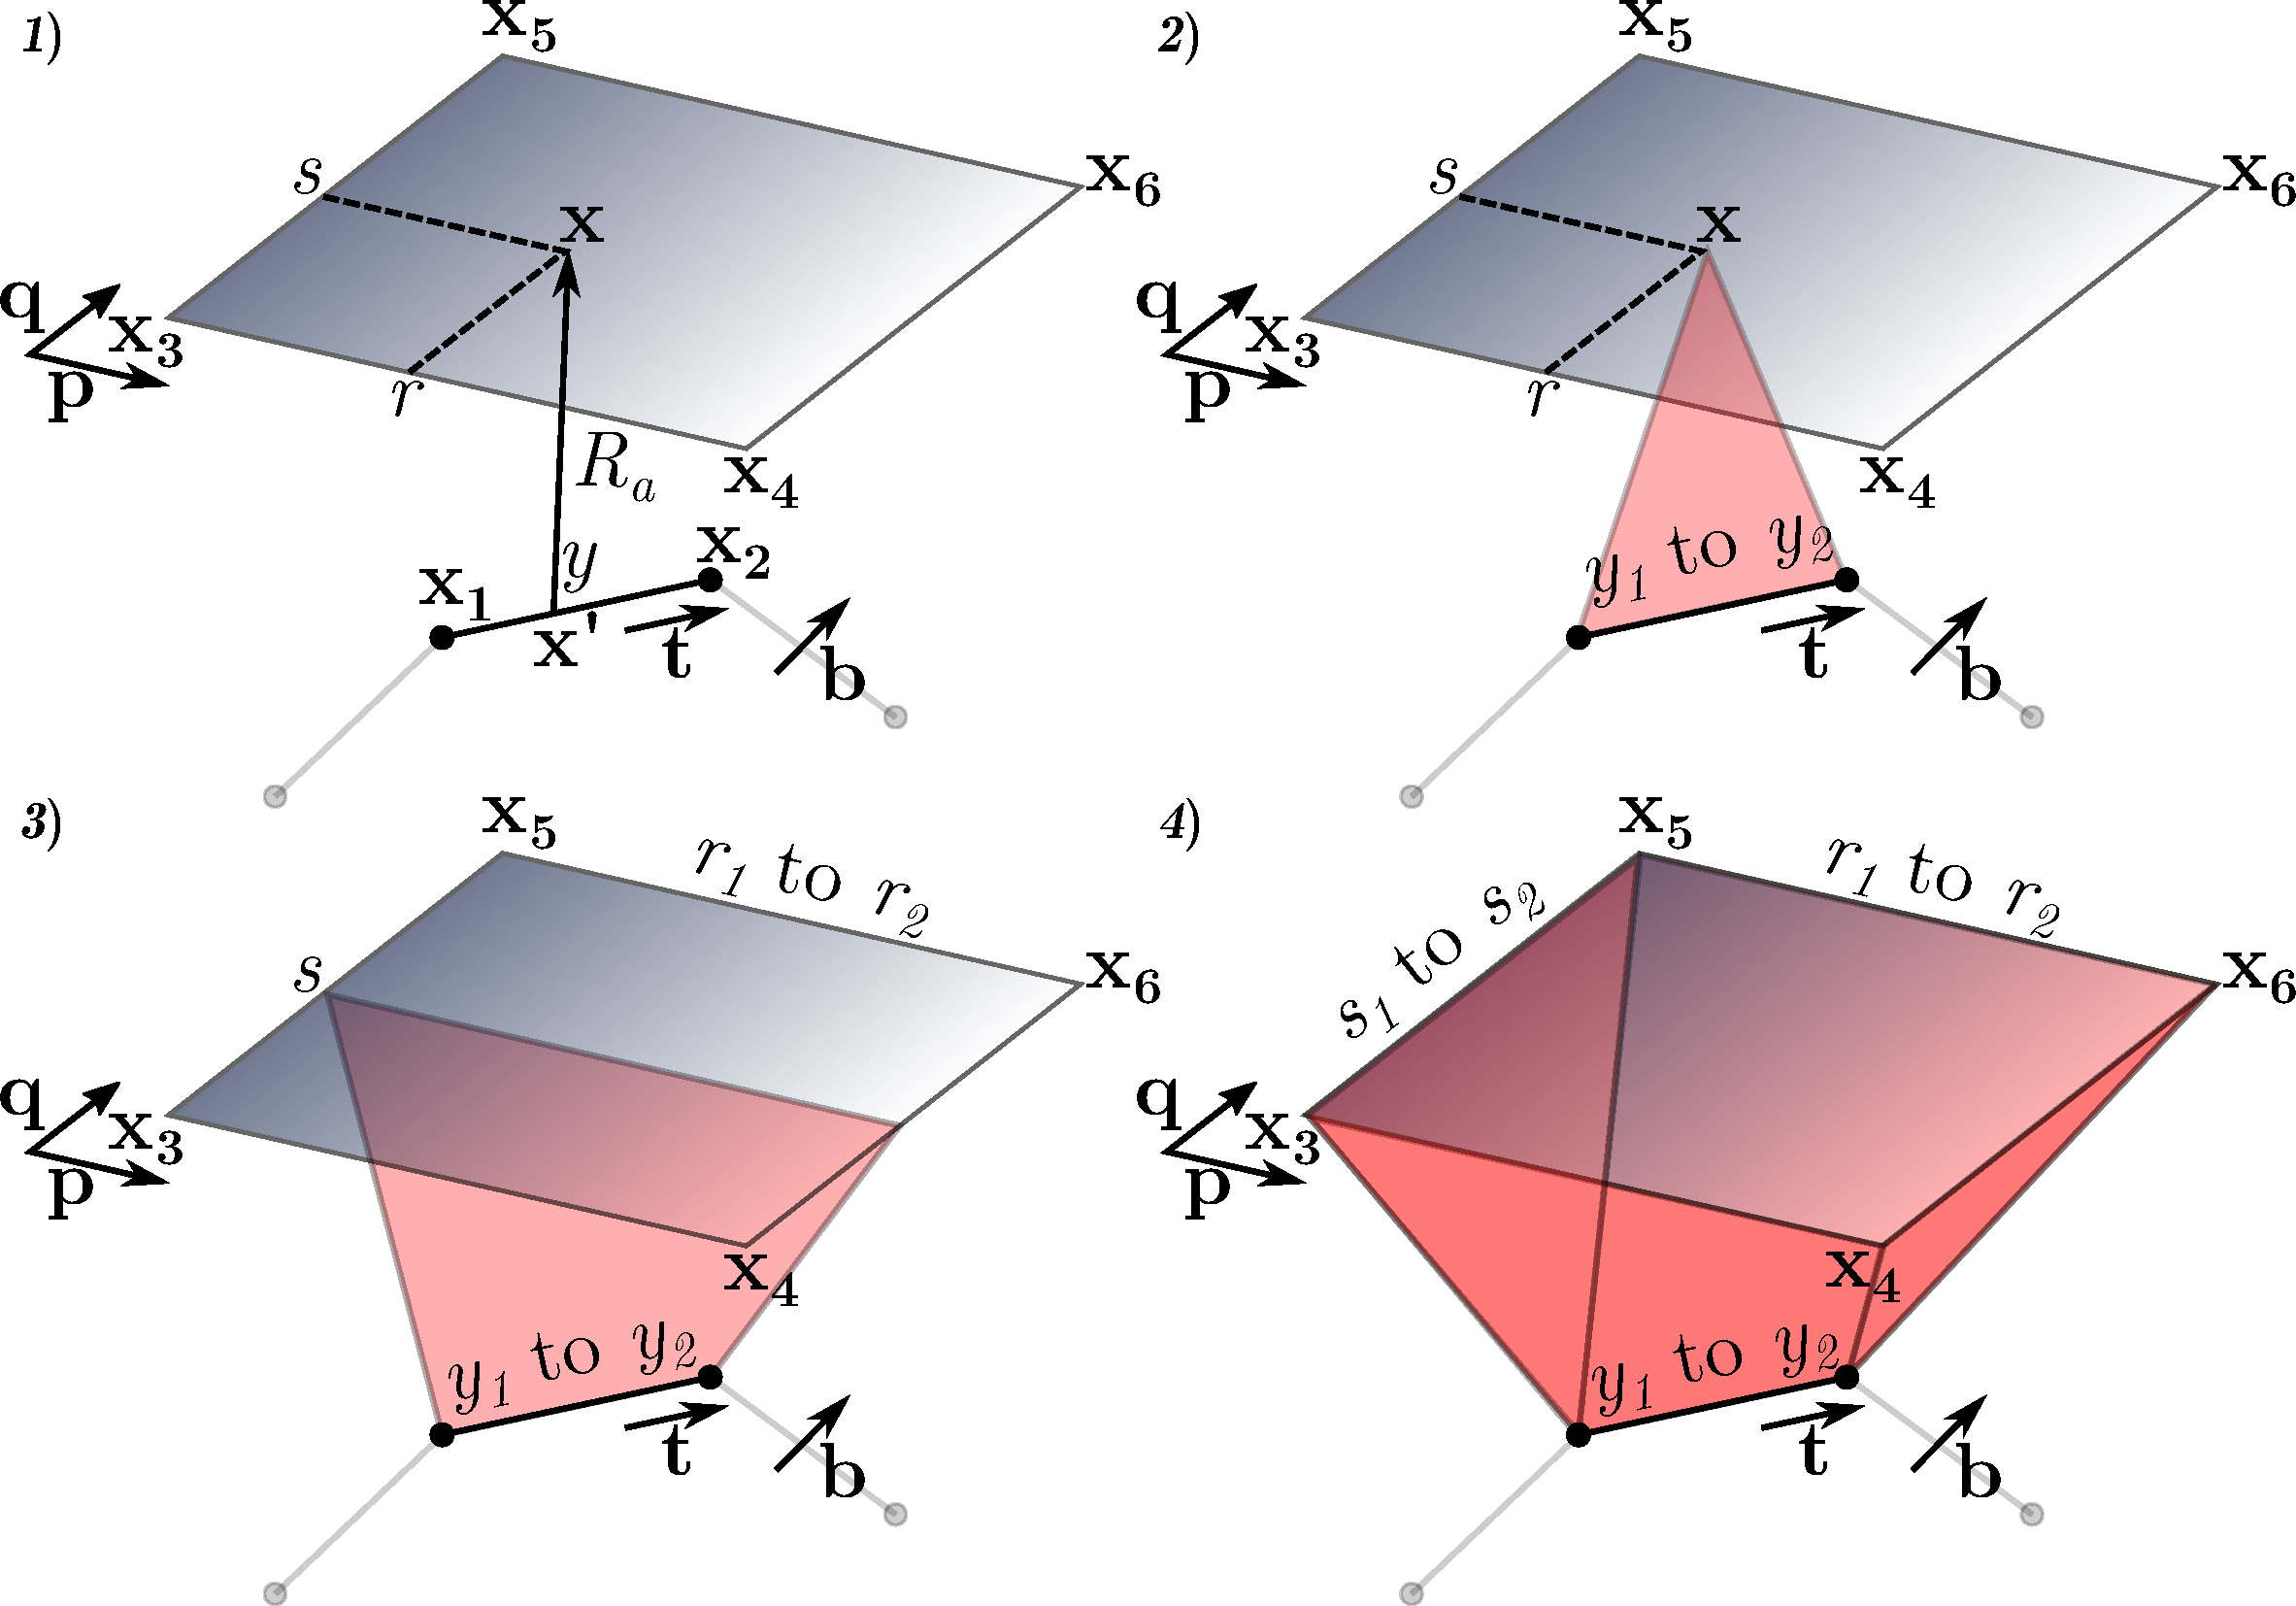
\includegraphics[width=\linewidth]{force_calc.pdf}
			\captionof{figure}{Series of line integrals that were solved analytically for rectangular surface elements \cite{analytical_integration_of_the_forces_induced_by_dislocations_on_a_surface_element}.
			\textit{1}) For any given point $ \bm{x} $ on the surface element and any given point $ \bm{x'}$ on the dislocation line segment, define distance $ R_{a} $.
			\textit{2}) Integrate from $ x_{1} \to x_{2} $ along the line direction $ \bm{t} $.
			\textit{3}) Integrate from $ r_{1} \to r_{2} $ along vector $ \bm{p} $.
			\textit{4}) Integrate from $ s_{1} \to s_{2} $ along vector $ \bm{q} $.}
			\label{f:force_calc}
		}{0cm}
	%
	\section{Objectives}
	%
		The primary objective of this project is to create an efficient, GPU implementation of the analytical solution for the forces exerted on a rectangular surface element by a dislocation ensemble. The secondary objective is to implement similar analytical solutions for quadratic triangular surface elements.
	%
	\section{Acknowledgements}
	%
		We would like to thank Sylvain Queyreau for his invaluable input on the project. This work was supported by the Consejo Nacional de Ciencia y Tecnologia, Fondo Sectorial CONACYT-Secretaria de Energia-Sustentabilidad Energetica Cuarto Periodo [291129]. This work was supported by the Engineering and Physical Sciences Research Council [EP/L01663X/1].
}
\bibliographystyle{unsrtnat}
\bibliography{bib}
\fimage{0.98\paperwidth}{footer.pdf}
\end{multicols}
\end{document}